

%----------------------------------------------------------------------------------------
%	PACKAGES AND OTHER DOCUMENT CONFIGURATIONS
%----------------------------------------------------------------------------------------

\documentclass[12pt]{article} % A4 paper and 11pt font size
\usepackage{natbib}
\usepackage{hyperref}
\usepackage{graphicx}
%\usepackage{fourier}
\usepackage{geometry}
 \geometry{
 a4paper,
 total={210mm,210mm},
 left=20mm,
 right=20mm,
 top=20mm,
 bottom=20mm,
 }
\title{Assignment 4}
\author{Victor Dasari} % Your name

\date{\normalsize\today}


%----------------------------------------------------------------------------------------
%	TITLE SECTION
%----------------------------------------------------------------------------------------

 % Today's date or a custom date

\begin{document}
\newpage


%----------------------------------------------------------------------------------------
%	PROBLEM 1
%----------------------------------------------------------------------------------------

\section{Q1}
In this question I've been asked to find the Jaccard distance for unigrams,bigrams and trigrams for the links successfully processed with boilerpipe during assignment three and the links successfully processed with boilerpipe during assignment four.
Below are the links that have been used for this question.
I processed links with boilerpipe during assignment 3 on 4/3/2015 and again on 4/24/2015. There is a 21 day time difference.
I've computed jaccard distance and not jaccard index. I first found the union and intersection, divided intersection with union and subtracted the result from 1 to get the jaccard distance.

Ex 1) http://www.thedailybeast.com/articles/2015/02/11/gates-foundation-ceo-vaccines-are-the-closest-thing-we-have-to-a-miracle.html
For the above link, the Jaccard distance for unigrams is .048
Jaccard distance for bigrams is .084
Jaccard distance for trigrams is .117

Ex 2) http://www.aljazeera.com/news/2015/02/students-murdered-university-north-carolina-campus-150211093231033.html
The jaccard distance for unigrams is .041, for bigrams is .066 and for trigrams is .083

Ex 3) \url{http://www.bbc.co.uk/news/world-us-canada-31433277#sa-ns_mchannel=rss&ns_source=PublicRSS20-sa?utm_source=twitterfeed&utm_medium=twitter}
The jaccard distance for unigrams, is 0, for bigrams is 0 and for trigrams is 0.

To generate unigrams, bigrams and trigrams I wrote three java scripts. One each for unigrams, bigrams and trigrams. 

%\lipsum[2] % Dummy text

%------------------------------------------------

%\subsection{Heading on level 2 (subsection)}



%------------------------------------------------

%\subsubsection{Heading on level 3 (subsubsection)}

%\lipsum[3] % Dummy text

%\paragraph{Heading on level 4 (paragraph)}

%\lipsum[6] % Dummy text

%----------------------------------------------------------------------------------------
%	PROBLEM 2
%----------------------------------------------------------------------------------------
\section{Q2}
I've generated timemaps for about 8000 links out of the total 10000 links. I've uploaded these to github. They are in the timemaps folder. Many of these returned 404 responses. I've used wget to generate the timemaps and have restricted the number of tries to only one to save time.
I've used R to plot the cumulative distributive function of number of mementos and the number of links.
For mementos, generated using wayback.archive-it.org there is no http in the  beginning of the URI.So I again had to add "http:" for such links. 

Ex of such a memento:
"uri":"//wayback.archive-it.org/all/20111208020033/http://www.radford.edu/

\begin{figure}
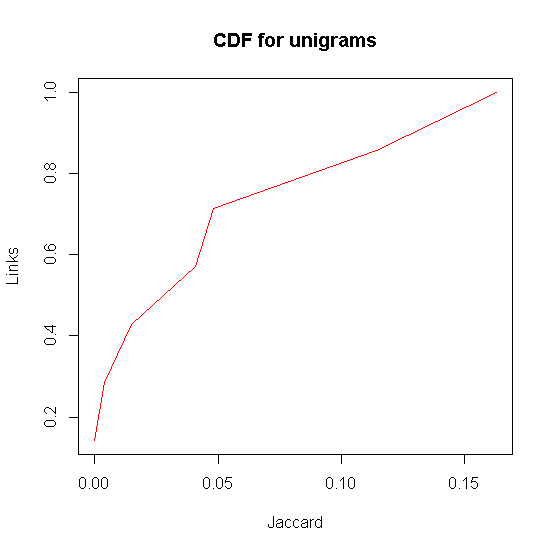
\includegraphics[width=.5\textwidth]{cdf-uni.png}
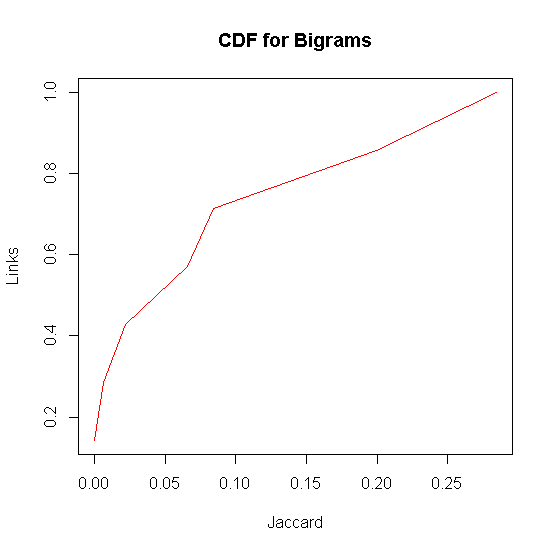
\includegraphics[width=.5\textwidth]{cdf-bi.png}
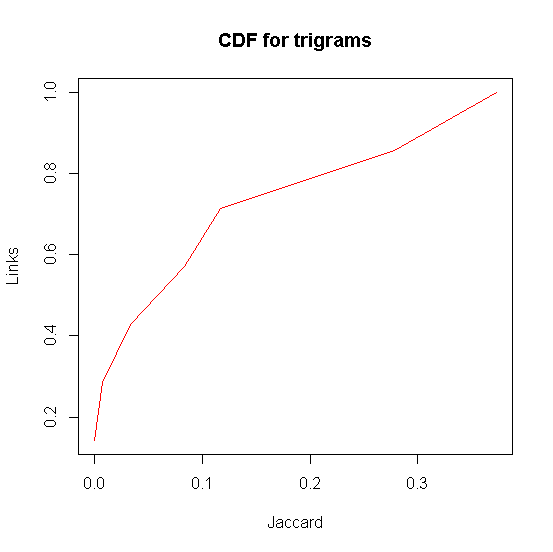
\includegraphics[width=.5\textwidth]{cdf-tri.png}
\caption{Graphs for question 1}
\end{figure}

\begin{figure}
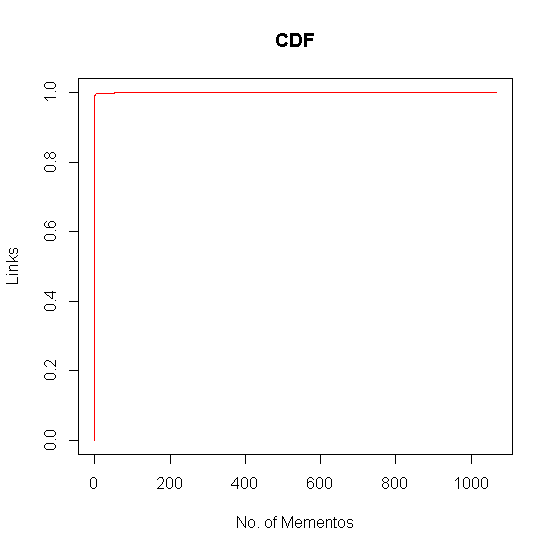
\includegraphics[width=.8\textwidth]{cdf-q2.png}
\caption{CDF for question 2}
\end{figure}

\section{Q3}
I've hand picked 20 urls that have greater than 20 mementos. Below is the list of 20 urls used 

1)www.odu.edu

2)www.nsu.edu

3)www.cs.odu.edu

4)www.vuu.edu

5)www.hamptonu.edu

6)www.hsc.edu

7)www.hollins.edu

8)www.stratford.edu

9)www.ecpi.edu

10)www.gmu.edu

11)www.vcu.edu

12)www.emu.edu

13)www.liberty.edu

14)www.marymount.edu

15)www.longwood.edu

16)www.radford.edu

17)www.su.edu

18)www.regent.edu

19)www.cnu.edu

20)www.cnn.edu

All the above links have mementos greater than 20 and the first mementos are before the year 2013.
I then used a Trial2.java code which takes all the links of mementos as input and outputs the boiler pipe results in different files. These files are again given as input to another java file that generates unigrams and stores these in different files. These files are given as input to two shell scripts inter.sh and union.sh which output the intersection and union values for the first memento and every other memento. \cite{inter}I then calculated the jaccard distance in excel and assigned the corresponding date time value to each jaccard distance value. I then used these 20 excel sheets plotted 19 graphs in R. For regent.edu when I processed the first memento through boiler pipe I got the following 504 response code which is why I do not have a graph for it.

---------------------
504 Gateway Time-out

The gateway did not receive a timely response from the upstream server or application. Sorry for the inconvenience.
Please report this message and include the following information to us.
Thank you very much!

URL:	http://web.archive.org/web/19970711013713/http://www.regent.edu/
Server:	wwwb-front1.us.archive.org
Date:	2015/05/01 00:42:14
------------------------

I used this link to generate the timemaps, http://labs.mementoweb.org/timemap/json/.
\cite{time}
The following graphs have the same heading. I later realized that its hard to differentiate between graphs because of this. I wish I had changed them before running the R script.

\begin{figure}
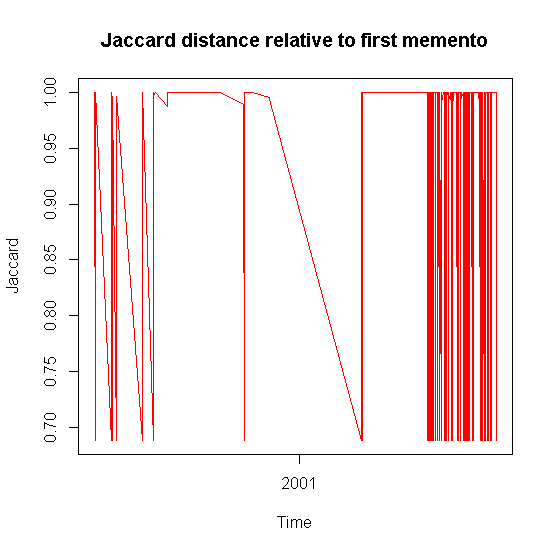
\includegraphics[width=3in]{cnn-graph.png}
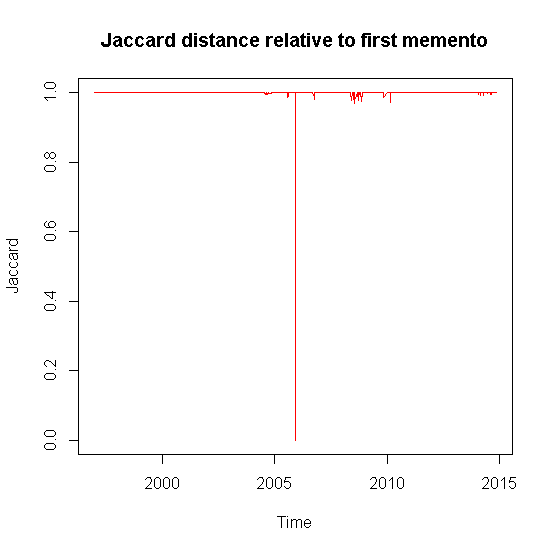
\includegraphics[width=3in]{cnu-graph.png}
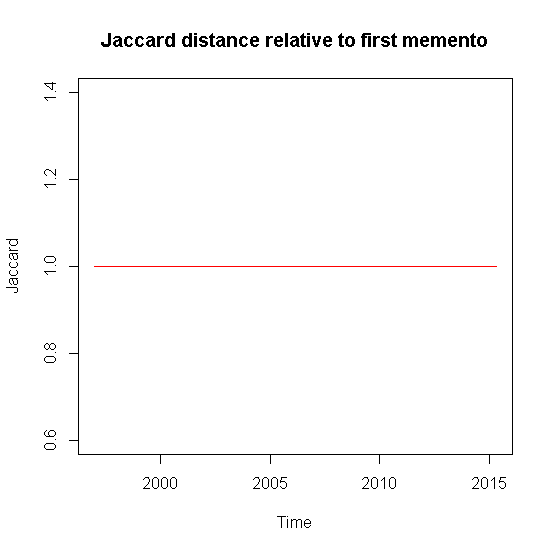
\includegraphics[width=3in]{cs-odu.png}
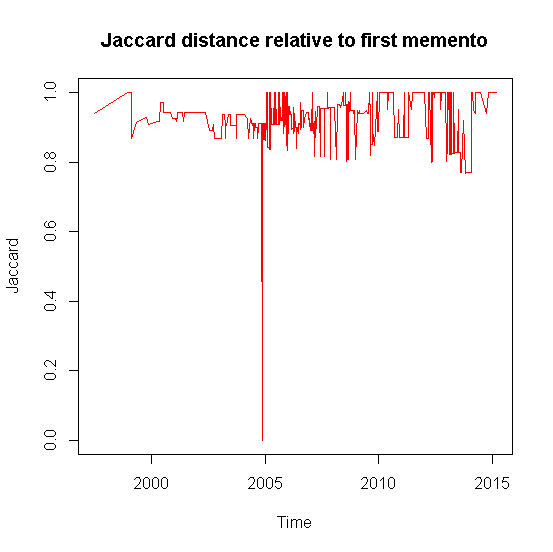
\includegraphics[width=3in]{ecpi-graph.png}
\caption{Graphs for cnn.com, cnu.edu, cs.odu.edu, ecpi.edu}
\end{figure}

\begin{figure}
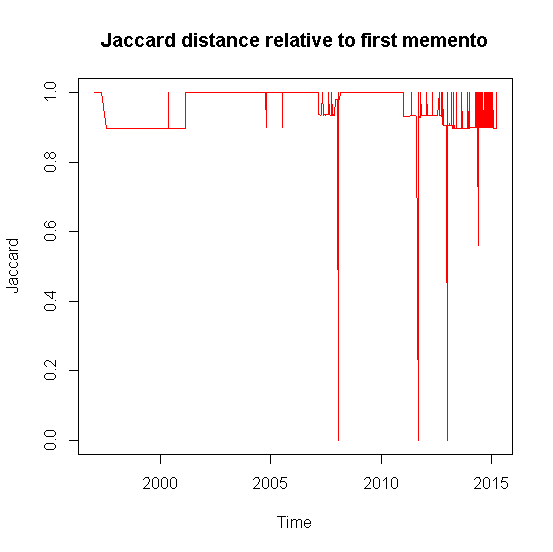
\includegraphics[width=3in]{emu-graph.png}
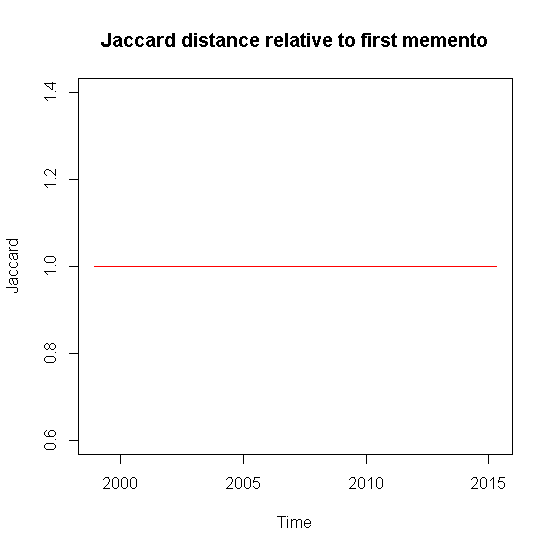
\includegraphics[width=3in]{gmu-graph.png}
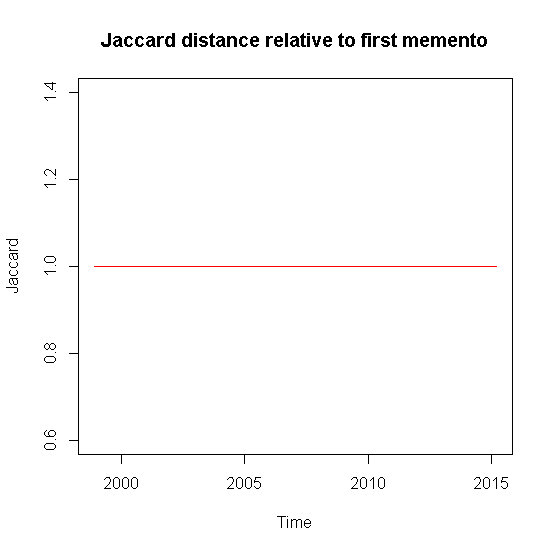
\includegraphics[width=3in]{hampton-graph.png}
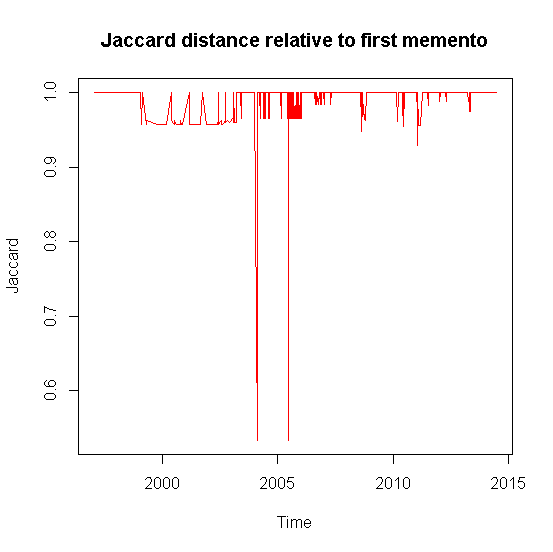
\includegraphics[width=3in]{hollins-graph.png}
\caption{Graphs for emu.edu, gmu.edu, hamptonu.edu, hollins.edu}
\end{figure}

\begin{figure}
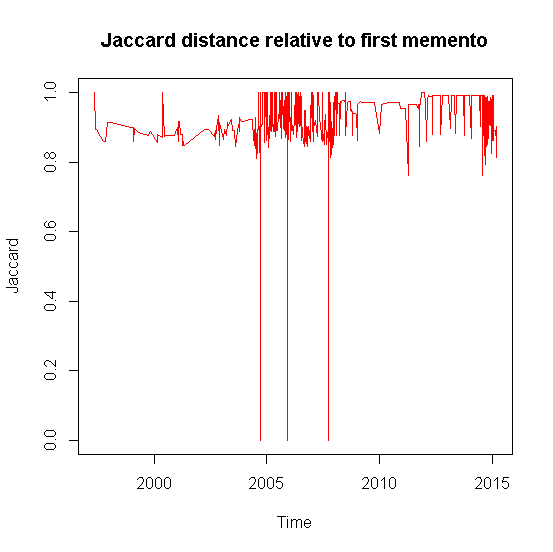
\includegraphics[width=3in]{hsc-graph.png}
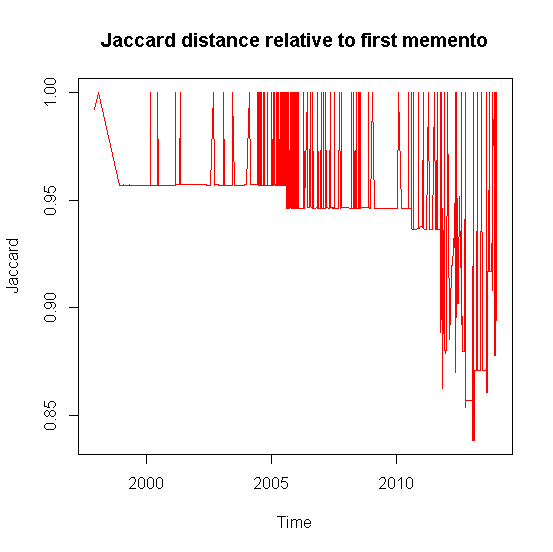
\includegraphics[width=3in]{liberty-graph.png}
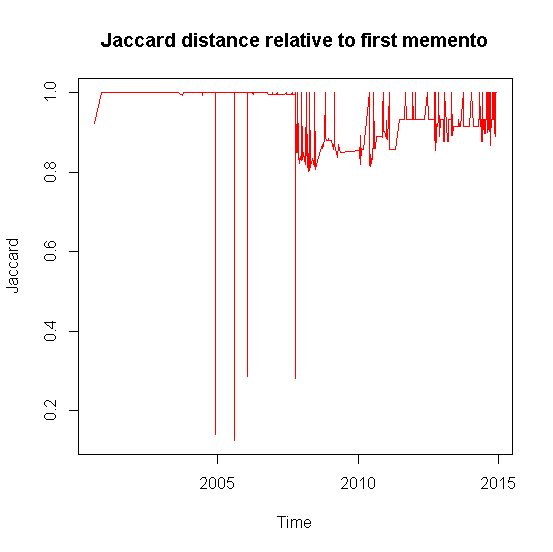
\includegraphics[width=3in]{long-graph.png}
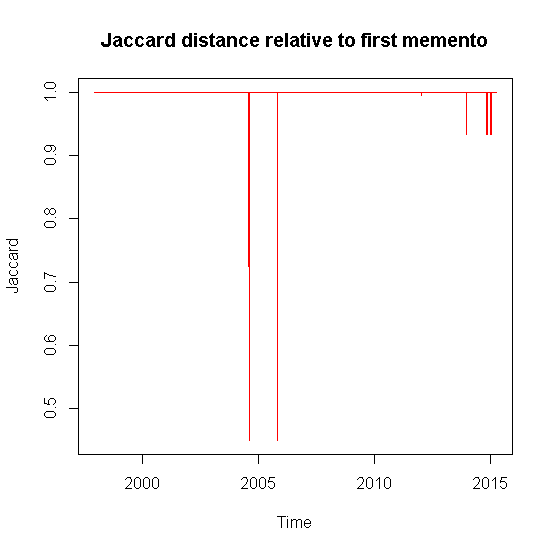
\includegraphics[width=3in]{mary-graph.png}
\caption{Graphs for hsc.edu, liberty.edu,longwood.edu, marymount.edu}
\end{figure}

\begin{figure}
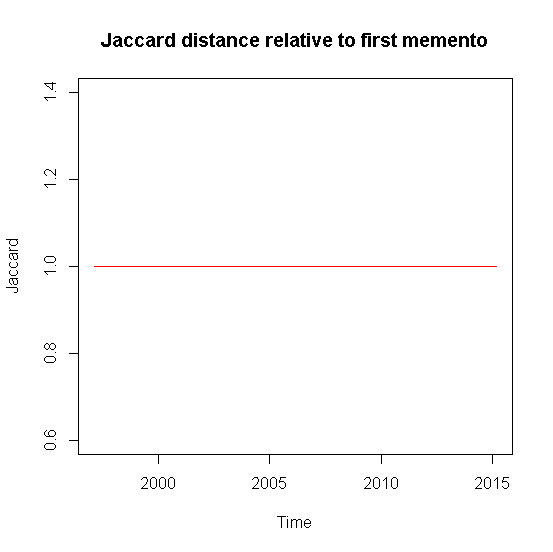
\includegraphics[width=3in]{nsu-graph.png}
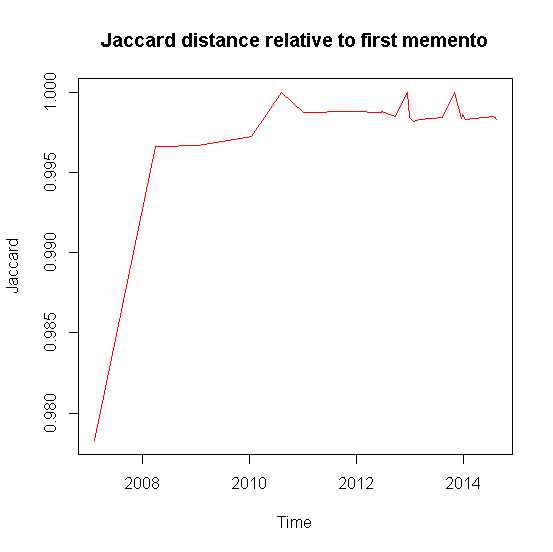
\includegraphics[width=3in]{odu-graph.png}
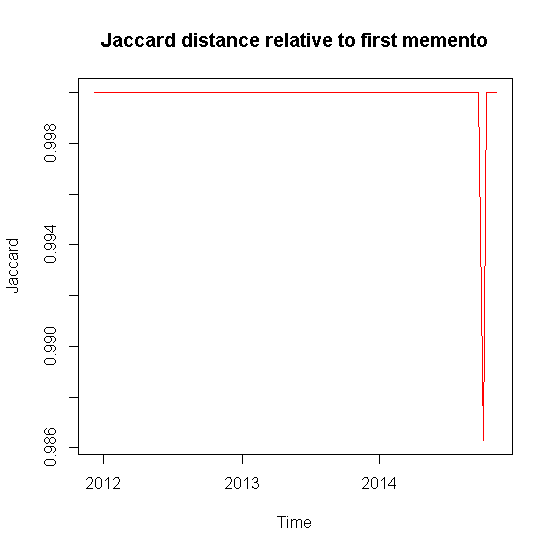
\includegraphics[width=3in]{rad-graph.png}
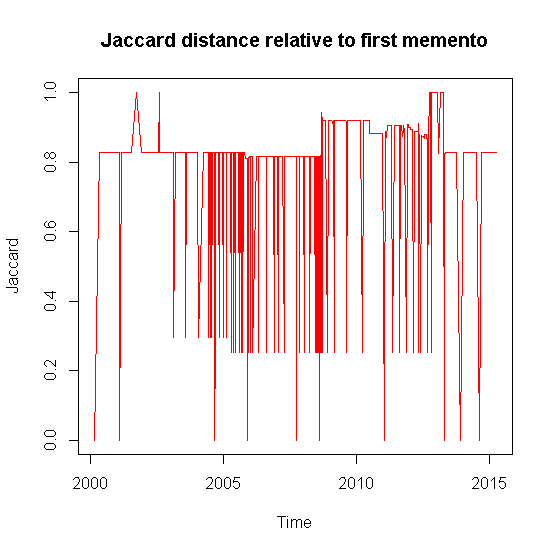
\includegraphics[width=3in]{strat-graph.png}
\caption{Graphs for nsu.edu, odu.edu, radford.edu, stratford.edu}
\end{figure}

\begin{figure}
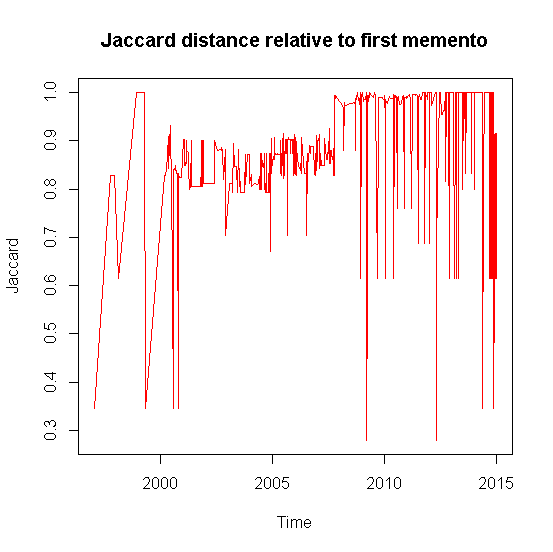
\includegraphics[width=3in]{su-graph.png}
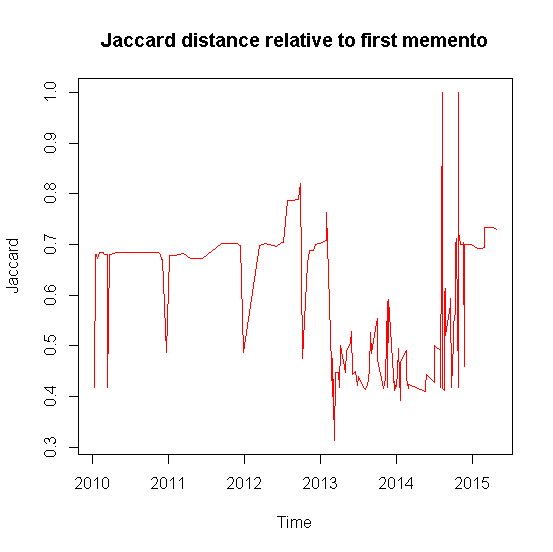
\includegraphics[width=3in]{vcu-graph.png}
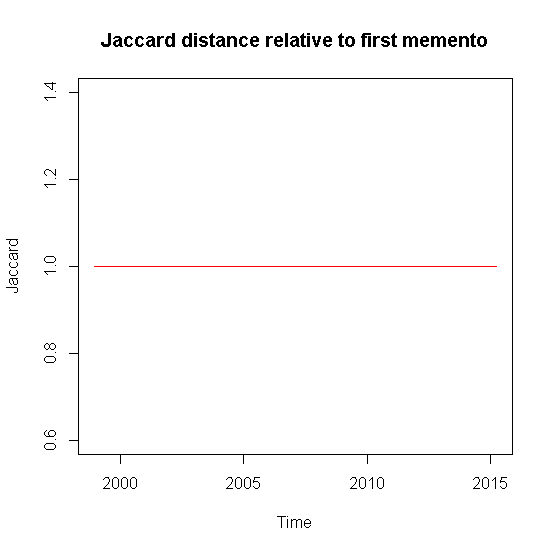
\includegraphics[width=3in]{vuu-graph.png}
\caption{Graphs for su.edu, vcu.edu, vuu.edu}
\end{figure}



\bibliographystyle{plain}
\bibliography{mybib}


%------------------------------------------------


%------------------------------------------------



%----------------------------------------------------------------------------------------

\end{document}